\section{Introduction}

\subsection{Motivation}

 Software analytics involved performing analysis of data collected during software development
 processes for software managers and engineers to gain insights into their projects
 to make better decisions and deliver high quality software~\cite{menzies2013software}.
 Thanks to the development in Internet and software engineering, there's huge amount
 of data generated from software projects. For example, at the time of this writing (Feb 2016),
 our web searches show that Mozilla Firefox has over 1.1 million bug reports, and
 platforms such as GitHub host over 14 million projects. The PROMISE repository
 of SE data has grown to 200+ projects~\cite{promise15} and this is just one of
 over a dozen open-source repositories that are readily available to researchers~\cite{rod12}.
 Although so much data is available, the useful and insightful information is always 
 hidden behind the project data, which means it's impossible to obtain by investigate the raw data manually by software researchers and practitioners due to the volume of the data. Therefore, some
 automatic and intelligent techniques are required to assist software analytics tasks.
 
 Over the past decade, data mining algorithms have become well
 recognized tools to explore software data to learn useful patterns or predictive
 models. Several tasks and practices within software development have been
 improved by applying results of software analytics, like requirement analysis, implementation,
 testing, building and maintenance\cite{xie2009data}.
%  For example, in software development process, bug
%  reports provide crucial information to developers to fix bugs and improve the
%  software quality. The issues with bug reports that many software teams faced
%  are how to eliminate duplicated reports, how to classify bug reports according
%  to priority, whether the bug reports provide sufficient information to reproduce,
%  and how to triage bug reports and find the right software engineers to fix the bug etc. 
%  Usually these tasks can be done by human beings spending a lot of time, but like
%  1.1 million bug reports in Mozilla Firefox, automation is very important and
%  necessary in this scenario. 
By using text data in software development, data mining algorithms like SVM, 
linear regression, Naive Bayes, K-nearest neighbors, Decision tree and other
algorithms have shown great power in addressing problems like
duplicate bug reports detection \cite{sun2010discriminative,jalbert2008automated,alipour2013contextual,nguyen2012duplicate},
bug reports classification \cite{antoniol2008bug,zanetti2013categorizing,lamkanfi2011comparing,tian2013drone}, 
bug report quality analysis \cite{bettenburg2008makes} and bug reports
triage\cite{anvik2006should, bhattacharya2010fine, lin2009empirical}. 
By using software development process data,
researchers can estimate project efforts\cite{dejaeger2012data,kocaguneli2012value, menzies2013local},
predict risks of development delay \cite{da2014empirical,choetkiertikul2015predicting}, 
and predict defective modules within projects\cite{me07b,hall11,lessmann2008benchmarking};
By mining security data within software context, software practitioners can predict identifiers of software vulnerabilities\cite{shin2011evaluating,scandariato2012predicting,medeiros2014automatic} by utilizing data mining algorithms like SVM, Naive Bayes, and
Random Forests to build 
predictive models. In all of these software analytics works,  most authors claim
their tools achieve pretty good performance or even better than the methods they compared to in terms
of some evaluation measures, like accuracy, F1-measure, and precision \cite{lamkanfi2011comparing, alipour2013contextual,lin2009empirical,lessmann2008benchmarking,hall11}.

Although data mining algorithms are core tools and extensively used in software analytics, software engineering 
researchers rarely develop their own versions of algorithms from scratch. Instead, they use
open source software tools like  
Scikit-learn(Python)\cite{scikit-learn}, Weka(Java)\cite{hall2009weka}, and numerous data mining packages in R. Thanks to those open 
source tools, they alleviate the burden of coding up those classic data mining algorithms and make
software researchers' life easy. However, this sort of convenience might put 
software analytics at risk because researchers tend to put lots of efforts on tasks like problem formalization, 
data collection and data processing and then simply use data mining tool as a black box to build 
predictive models without any further considerations on data mining algorithms\cite{sun2010discriminative,jalbert2008automated, antoniol2008bug,zanetti2013categorizing,lamkanfi2011comparing,tian2013drone, alipour2013contextual,lin2009empirical,hall11,me07b,choetkiertikul2015predicting,anvik2006should, bhattacharya2010fine}.
Different implementations might
provide different tuning parameters, which control the behavior of learners to explore the data.
Take Random Forests classifier for example.
By comparing three implementations in Weka\footnote {http://goo.gl/hqol4H}, 
Scikit-learn\footnote{http://goo.gl/Lfi3IH} and R package\footnote{https://goo.gl/ht4pZ1}, 
it's observed that, on one hand, they have different sets of built-in tuning parameters
to control the algorithms. That means software analytics results obtained by
using one tool might not be easily reproduced by using the other one.
On the other hand, even thought they all have similar parameters to control
the same behavior, like number of trees, the default values vary a lot, like
10, 100 and 500 in Scikit-learn, Weka, and R package. 
Those different values will change the the behavior of a data miner, 
to some degree, and finally change the results of the learner.


% \bi
% \item {\em -I}: the number of trees (default: 100).
% \item {\em -K}: the number of features (default: unlimited).
% \item {\em depth}: the maximum depth of the trees (default: unlimited).
% \item {\em -B}: break ties randomly when several attributes look equally good.
% \item {\em -S}: the seed for random number generator (default:1).
% \ei

% In Scikit-learn, we have the following parameters to control Random Forests behavior\footnote{http://goo.gl/Lfi3IH}:

% \bi
% \item {\em n\_estimators}: the number of trees (default: 10)
% \item {\em max\_features}: the number of features (default: $\sqrt{n\_features}$, options: log2(n\_feautres), etc).
% \item {\em max\_depth}: the maximum depth of the trees (default: nodes are expanded all leaves are pure or until all leaves contain less than min\_samples\_split samples).
% \item {\em min\_samples\_split}: the minimum number of samples required to split an node (default: 2).
% \item {\em min\_samples\_leaf}: the minimum number of samples in newly created leaves (default:1)
% \item {\em random\_state}: the seed for random number generator(default:numpy.random).
% \ei

% In randomForest R package, we have the following parameters \footnote{https://goo.gl/ht4pZ1}:
% \bi
% \item {\em ntree}:  the number of trees to grow (default:500).
% \item {\em mtry}: the number of features randomly sampled as candidates at each split (default: ${\sqrt{n\_features}}$).
% \item {\em nodesize}: minimum size of terminal nodes (default: 5).
% \item {\em maxnodes}: maximum number of terminal nodes trees in the forest can have(default: unlimited).
% \ei

% By looking at the tuning parameters for these three different versions of Random Forest, 

One of the ``black arts'' of data mining is setting the tuning
parameters that control the choices within a data miner. 
Nevertheless, we rarely tuned our predictors in
any software analytics tasks since we reasoned that a data miner's default tunings have been 
well-explored by the developers of those algorithms (in which case
tuning would not lead to large performance improvements). Also, we suspected that
tuning would take so long time and be so CPU intensive that the benefits gained would not be worth effort.

However, there are a few work within the domain of software analytics, studying 
the impacts of parameters in learning algorithm. Corazza et al.\cite{corazza2010effective} 
explore hyper-parameter space of support vector regression (SVR) running tabu-search to perform parameter tuning, which improves the performance of effort estimator. However, 
tabu-search might not be suited to the optimisation of models
with continuous variables and of higher dimensionality 
(e.g. having five or more independent management options to
investigate) \cite{mayer1998tabu}. Lessmann et al.\cite{lessmann2008benchmarking}
tuned parameters for some of their defect predictors using  a {\em grid search}.
Similarly, Tantithamthavorn et at.\cite{tantithamthavorn2016automated} 
applied {\em caret} package \cite{kuhn2008caret}, which is a grid-search 
based hyper-parameter optimization package in R,  to tune defect predictors.
To investigate the performance of grid search on parameter tuning, we
run a preliminary experiment where both grid searcha and DE are
used as tuners.
We find that grid search takes quite long time to find 
optimal parameters compared with DE\footnote{In this preliminary experiment, both methods achieve similar performance, but DE is much faster than grid search and more details will be discussed in our future SSBSE paper}, as shown in figure \ref{fig:grid_runtime}. 
The reason is that grid search explores a large searching space which is actually not necessary. 
This gives us a hint that  more simple and efficient tuning framework is needed for software analytics.
Furthermore, the impact of tunings seems not be widely acknowledged by
software analytics community, which is an important factor will(to some extent) change
the conclusion of software analytics based on previous work~\cite{mayer1998tabu,tantithamthavorn2016automated}.

\begin{figure}[h]
\begin{center}
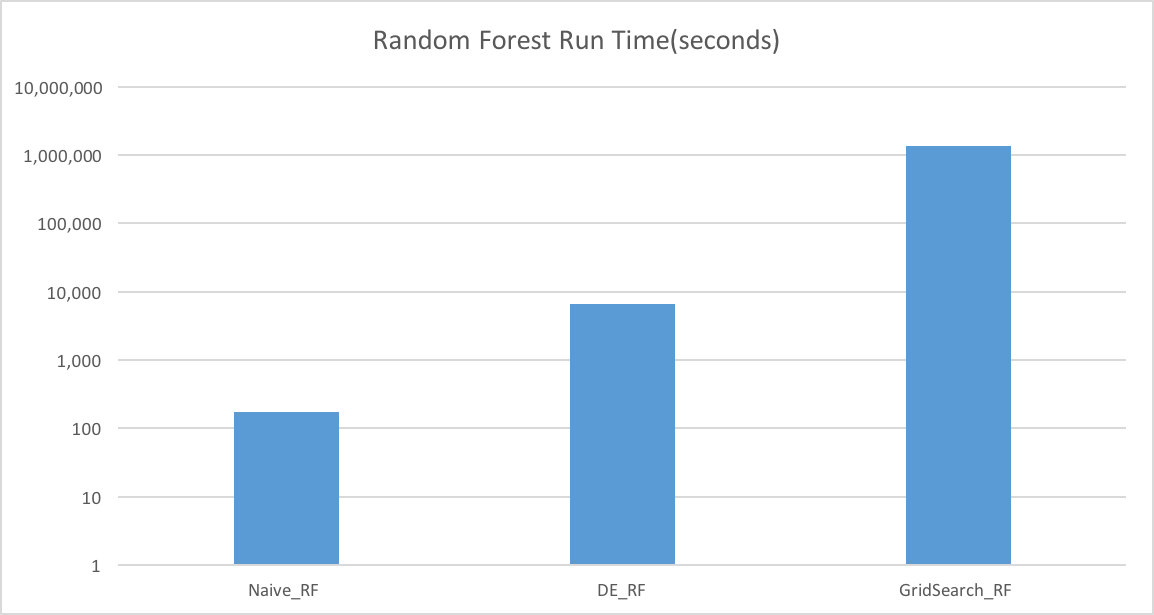
\includegraphics[width=6.5cm]{./eps/rf_runtime.png}
\end{center}
\caption{Compare overall run time of DE and grid search as tuners to tune random forest over defect prediction data.}\label{fig:grid_runtime}
\end{figure}

%  \begin{table}[!h]
% \renewcommand{\baselinestretch}{0.5}
% \renewcommand{\arraystretch}{3.5}
% \scriptsize
% \centering
%   \begin{tabular}{p{0.55cm}p{0.25cm}p{0.5cm}p{0.5cm}p{0.5cm}p{0.5cm}p{0.5cm}p{0.35cm}p{0.5cm}p{0.35cm}}\hline \hline
% %   \begin{tabular}{c c c c c c c c c c } \hline
%   Data &jm1&prop1&prop2&prop3&prop4&prop5&camel&xalan2.5&jdt
% \\\hline 
%   Caret &1845 &8342 &13850 &2183 &2213 &1379 &177 &300 &336\\\hline
%   DE  &598 &1099 &609 &514 &513 &513 &147 &156 &155
% \\\hline \hline
%   Data &pc5&pltfm2&pltfm21&pltfm3&debug3.4&swt3.4&mylyn&xalan2.6 & pde
% \\\hline 
%   Caret &888 &4422 &5523 &7782 &317  &294 &374  &294 & 431\\\hline
%   DE   &264 & 601 & 695 & 925 & 153 & 162 & 180 & 159 & 173 
% \\ \hline\hline
% \\  \end{tabular}

%   \caption{ Compare Running time of reproduced Tantithamthavorn et at.\cite{tantithamthavorn2016automated} work V.S. Differential Evolution(DE) in seconds
%   }\label{tab:grid_runtime}
% \end{table} 

To investigate the effect of parameter tuning on software analytics, 
we take defect prediction as an example to study how tuning
would change conclusions claimed by previous researchers. 
Since defect prediction has been explored so well during
the past years, tremendous works within this field make it as a very 
active field in software analytics. Furthermore, defect prediction
share many similarities with other software analytics tasks, 
like delay prediction, effort estimation and bug report classification,
in terms of utilizing data miners as its core tool. 
Therefore, in this paper, we study effect of tuning on defect prediction.

\subsection{Research Questions}
As a case study of 17 groups of defect prediction data sets from open source java system,  the research questions addressed in this paper are the following:

\bi
\item RQ1: {\bf{\em Does   tuning    improve the performance scores of a predictor?}} %We will show below
%  examples of truly dramatic improvement:
%  usually by 5 to 20\% and often by much more (in one extreme case,  precision improved from 0\% to 60\%).
\item RQ2: {\bf {\em Does tuning change conclusions on what learners are better than others?}} 
% Recent SE papers~\cite{lessmann2008benchmarking,hall11} claim that some learners are better than others. 
% Some of those conclusions are completely changed by tuning. 
\item RQ3: {\bf {\em Does tuning change conclusions about what factors are most important in software engineering?}} %Numerous recent SE papers (e.g.~\cite{bell2013limited,rahman2013how,me02k,Moser:2008,zimmermann2007predicting,%
% herzig2013predicting}) use data miners to conclude that {\em this}
% is more important than {\em that} for reducing software project defects.
% Given the  tuning results of this paper, we show that such conclusions need to be revisited.
\item  RQ4: {\bf {\em Is tuning easy?}} %We show that one of the simpler multi-objective optimizers
% (differential evolution~\cite{storn1997differential}) works very well for tuning defect predictors. 
\item RQ5: {\bf {\em Is tuning impractically slow?}} %We achieved dramatic improvements in the performance scores
% of our data miners in less than 100 evaluations (!); i.e., very
% quickly.
\item RQ6: {\bf{\em Should data miners be used ``off-the-shelf'' with their default tunings?}}
% For defect prediction from static code measures, our answer is an emphatic ``no'' (and
% the implication for other kinds of  analytics is now an open and urgent question).
\ei

\subsection{Contribution of this thesis}

Based on our answers to above research questions,  we strongly advise that:
\bi
\item
Data miners should not be used ``off-the-shelf'' with default tunings.
\item
Any future paper on defect prediction should include a 
tuning study. Here, we have found  an algorithm called differential
evolution to be a useful method for conducting such
tunings.
\item
Tuning needs to be repeated
whenever data or goals are changed.
Fortunately, the cost of finding good tunings is not excessive since, at least for
static code defect predictors, tuning is easy and fast.
\ei

\subsection{Statement of thesis}

The results of this paper show that, at least for
defect prediction from  code attributes, parameter tuning for defect predictors is {\em remarkably simple} and can {\em dramatically improve the performance}. 

\subsection{Publications (submitted) to date}

\bi
\item W. Fu, T. Menzies, X. Shen ``Tuning for Software Analytics: is it Really Necessary?'', Information and Software Technology, Elsevier, submitted.

\item JC. Nam, W. Fu, S. Kim, T. Menzies, L. Tan ``Heterogeneous Defect Prediction'', Transactions on Software Engineering, IEEE, submitted.
\ei

\subsection{Structure of this thesis}

The remainder of this paper is organized as follows. Section 2 reviews the literature on defect prediction, tuning in defect prediction , tuning algorithms and associated problems in recent work. Section 3 presents the data sets and  experiment design of our study . Section 4 discusses the results of our experiment. Section 5 discloses the reliability and validity of our study. Finally, section 6 draws the conclusion. Finally, section 7 discusses the next step and future work.
% Faced with this data overload,
% researchers in empirical SE
% use  data miners  to generate 
% {\em defect predictors from static code measures}.
% Such   measures can be
% automatically extracted from the code base, with very little effort
% even for very large software systems~\cite{nagappan05}. 



%Before beginning, we digress for one  clarification.
%This paper is {\em not} arguing that
%software analytics is somehow wrong-headed or misguided.
%In the age of the Internet and global access to software engineering data,
%there exists the  problem of information overload. {\em Something} must be %done to
%allow analysts to make conclusions via an automatic analysis over a lot of %data.
%The results of this paper is that for a particular local context
%(a specific data set and a specific goal) there exists  
%methods for optimizing the conclusions reached in that context.  
%Those conclusions
%may not generalize to other contexts but this  is not a council for despair. 
%As shown here, 
%there  exists general methods for finding
%local conclusions in a particular context. Further,
%those
%methods are  very simple to implement and very fast to execute.